\chapter{Backtracking}

\section{Regular Expression Matching} %%%%%%%%%%%%%%%%%%%%%%

\subsubsection{Description}
Implement regular expression matching with support for \fn{'.'} and \fn{'*'}.

\fn{'.'} Matches any single character.
\fn{'*'} Matches zero or more of the preceding element.

The matching should cover the entire input string (not partial).

Some examples:
\begin{Code}
isMatch("aa","a") → false
isMatch("aa","aa") → true
isMatch("aaa","aa") → false
isMatch("aa", "a*") → true
isMatch("aa", ".*") → true
isMatch("ab", ".*") → true
isMatch("aab", "c*a*b") → true
\end{Code}

\subsubsection{Solution}

\begin{Code}
public boolean isMatch(String s, String p) {
    if (p.isEmpty()) {
        return s.isEmpty();
    } else if (p.length() == 1) {
        return s.length() == 1 && isEqual(s, p);
    } else if (p.charAt(1) != '*') {
        return s.length() > 0 && isEqual(s, p) && isMatch(s.substring(1), p.substring(1));
    } else {
        if (s.length() > 0 && isEqual(s, p)) {
            return isMatch(s, p.substring(2)) || isMatch(s.substring(1), p);
        } else {
            return isMatch(s, p.substring(2));
        }
    }
}

private boolean isEqual(String s, String p) {
    return s.charAt(0) == p.charAt(0) || p.charAt(0) == '.';
}
\end{Code}

\newpage

\section{Wildcard Matching}

\subsubsection{Description}
Implement wildcard pattern matching with support for \fn{'?'} and \fn{'*'}.

\fn{'?'} Matches any single character.
\fn{'*'} Matches any sequence of characters (including the empty sequence).

\begin{Code}
Some examples:
isMatch("aa","a") → false
isMatch("aa","aa") → true
isMatch("aaa","aa") → false
isMatch("aa", "*") → true
isMatch("aa", "a*") → true
isMatch("ab", "?*") → true
isMatch("aab", "c*a*b") → false
\end{Code}

\subsubsection{Solution}
\begin{Code}
public boolean isMatch2(String s, String p) {
    int is = 0, ip = 0, ks = -1, kp = -1;

    while (is < s.length()) {
        if (ip < p.length() && (s.charAt(is) == p.charAt(ip) || p.charAt(ip) == '?')) {
            is++;
            ip++;
        } else if (ip < p.length() && p.charAt(ip) == '*') {
            ks = is;
            kp = ip;
            ip++;
        } else if (kp != -1) {
            is = ++ks;
            ip = kp + 1;
        } else {
            return false;
        }
    }

    for ( ; ip < p.length() && p.charAt(ip) == '*'; ip++);
    return ip == p.length();
}
\end{Code}

\newpage

\section{Letter Combinations of a Phone Number}

\subsubsection{Description}
Given a digit string, return all possible letter combinations that the number could represent.

A mapping of digit to letters (just like on the telephone buttons) is given below.

\begin{center}
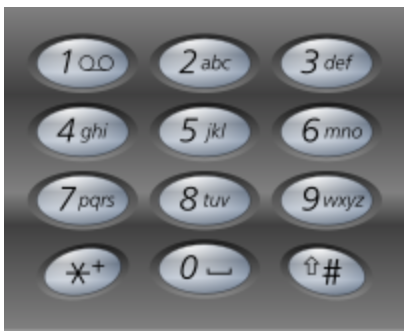
\includegraphics[width=150pt]{phone.png}\\
\figcaption{Phone Keyboard}\label{fig:phone-keyboard}
\end{center}

\textbf{Input:} Digit string \code{"23"}

\textbf{Output:} \code{["ad", "ae", "af", "bd", "be", "bf", "cd", "ce", "cf"]}.

\subsubsection{Solution}

\begin{Code}
private final String[] ARR = {
        "", "", "abc", "def", "ghi", "jkl", "mno", "pqrs", "tuv", "wxyz"
};

public List<String> letterCombinations(String digits) {
    List<String> list = new LinkedList<>();
    if (!digits.isEmpty()) {
        helper(digits, 0, list, "");
    }
    return list;
}

private void helper(String digits, int start, List<String> list, String s) {
    if (start >= digits.length()) {
        list.add(s);
        return;
    }
    int n = digits.charAt(start) - '0';
    for (char c : ARR[n].toCharArray()) {
        helper(digits, start + 1, list, s + c);
    }
}

public List<String> letterCombinations2(String digits) {
    LinkedList<String> queue = new LinkedList<String>();
    if (digits.length() == 0) {
        return queue;
    }

    Queue<String> next = new LinkedList<>();
    queue.add("");

    for (int i = 0; i < digits.length() && !queue.isEmpty(); ) {
        String s = queue.poll();
        int n = digits.charAt(i) - '0';
        for (char c : ARR[n].toCharArray()) {
            next.add(s + c);
        }
        if (queue.isEmpty()) {
            queue.addAll(next);
            next.clear();
            i++;
        }
    }
    return queue;
}
\end{Code}

\newpage

\section{Generate Parentheses}

\subsubsection{Description}
Given n pairs of parentheses, write a function to generate all combinations of well-formed parentheses.

For example, given \code{n = 3}, a solution set is:
\begin{Code}
[
  "((()))",
  "(()())",
  "(())()",
  "()(())",
  "()()()"
]
\end{Code}

\subsubsection{Solution}

\begin{Code}
public List<String> generateParenthesis(int n) {
    List<String> result = new LinkedList<String>();
    dfs(result, n, "", 0, 0);
    return result;
}

private void dfs(List<String> result, int n, String str, int left, int right) {
    if (left == n && right == n) {
        result.add(str);
        return;
    }
    if (left > n || right > n || left < right) {
        return;
    }
    dfs(result, n, str + "(", left + 1, right);
    dfs(result, n, str + ")", left, right + 1);
}
\end{Code}

\newpage

\section{Permutations}

\subsubsection{Description}
Given a collection of distinct numbers, return all possible permutations.

For example, \code{[1,2,3]} have the following permutations:
\begin{Code}
[
  [1,2,3],
  [1,3,2],
  [2,1,3],
  [2,3,1],
  [3,1,2],
  [3,2,1]
]
\end{Code}

\subsubsection{Solution}
\begin{Code}
public List<List<Integer>> permute(int[] nums) {
    List<List<Integer>> result = new ArrayList<List<Integer>>();
    permute(nums, result, 0);
    return result;
}

public void permute(int[] nums, List<List<Integer>> result, int start) {
    if (start >= nums.length) {
        List<Integer> list = new ArrayList<Integer>();
        for (Integer n : nums) {
            list.add(n);
        }
        result.add(list);
    }

    for (int i = start; i < nums.length; i++) {
        swap(nums, start, i);
        permute(nums, result, start + 1);
        swap(nums, start, i);
    }
}

public static void swap(int[] nums, int left, int right) {
    int temp = nums[left];
    nums[left] = nums[right];
    nums[right] = temp;
}
\end{Code}

\newpage

\section{Word Search}

\subsubsection{Description}
Given a 2D board and a word, find if the word exists in the grid.

The word can be constructed from letters of sequentially adjacent cell, where adjacent cells are those horizontally or vertically neighboring. The same letter cell may not be used more than once.

For example,
Given board =
\begin{Code}
[
  ['A','B','C','E'],
  ['S','F','C','S'],
  ['A','D','E','E']
]
\end{Code}

word = \code{"ABCCED"}, -> returns true,

word = \code{"SEE"}, -> returns true,

word = \code{"ABCB"}, -> returns false.

\subsubsection{Solution}

\begin{Code}
public boolean exist(char[][] board, String word) {
    for (int i = 0; i < board.length; i++) {
        for (int j = 0; j < board[0].length; j++) {
            if (dfs(board, i, j, word, 0)) {
                return true;
            }
        }
    }
    return false;
}

private boolean dfs(char[][] board, int i, int j, String word, int start) {
    if (start == word.length()) {
        return true;
    }
    if (i < 0 || i >= board.length || j < 0 || j >= board[0].length) {
        return false;
    }
    if (board[i][j] != word.charAt(start)) {
        return false;
    }

    board[i][j] ^= '#';
    boolean flag = dfs(board, i + 1, j, word, start + 1)
            || dfs(board, i - 1, j, word, start + 1)
            || dfs(board, i, j + 1, word, start + 1)
            || dfs(board, i, j - 1, word, start + 1);
    board[i][j] ^= '#';
    return flag;
}
\end{Code}

\newpage

\section{Word Search II}

\subsubsection{Description}
Given a 2D board and a list of words from the dictionary, find all words in the board.

Each word must be constructed from letters of sequentially adjacent cell, where adjacent cells are those horizontally or vertically neighboring. The same letter cell may not be used more than once in a word.

For example,
Given words = \code{["oath","pea","eat","rain"]} and board =
\begin{Code}
[
  ['o','a','a','n'],
  ['e','t','a','e'],
  ['i','h','k','r'],
  ['i','f','l','v']
]
\end{Code}
Return \code{["eat","oath"]}.

Note:
You may assume that all inputs are consist of lowercase letters a-z.

You would need to optimize your backtracking to pass the larger test. Could you stop backtracking earlier?

If the current candidate does not exist in all words' prefix, you could stop backtracking immediately. What kind of data structure could answer such query efficiently? Does a hash table work? Why or why not? How about a Trie? If you would like to learn how to implement a basic trie, please work on this problem: Implement Trie (Prefix Tree) first.

\subsubsection{Solution}

\begin{Code}
private class Trie {
    Trie[] nodes = new Trie[26];
    String word;
}

private void buildTrie(Trie trie, String word) {
    for (int i = 0; i < word.length(); i++) {
        if (trie.nodes[word.charAt(i) - 'a'] == null) {
            trie.nodes[word.charAt(i) - 'a'] = new Trie();
        }
        trie = trie.nodes[word.charAt(i) - 'a'];
    }
    trie.word = word;
}
\end{Code}

\newpage

\begin{Code}

public List<String> findWords(char[][] board, String[] words) {
    Trie trie = new Trie();
    for (String word : words) {
        buildTrie(trie, word);
    }
    Set<String> set = new HashSet<String>();
    for (int i = 0; i < board.length; i++) {
        for (int j = 0; j < board[0].length; j++) {
            dfs(set, board, i, j, trie);
        }
    }
    return new LinkedList<String>(set);
}

private void dfs(Set<String> set, char[][] board, int i, int j, Trie trie) {
    if (i < 0 || i >= board.length || j < 0 || j >= board[0].length) {
        return;
    }
    if (trie == null) {
        return;
    }
    char c = board[i][j];
    if (c < 'a' || c > 'z') {
        return;
    }
    trie = trie.nodes[c - 'a'];
    if (trie == null) {
        return;
    }
    if (trie.word != null) {
        set.add(trie.word);
    }

    board[i][j] ^= '#';
    dfs(set, board, i + 1, j, trie);
    dfs(set, board, i - 1, j, trie);
    dfs(set, board, i, j + 1, trie);
    dfs(set, board, i, j - 1, trie);
    board[i][j] ^= '#';
}
\end{Code}

\newpage

\section{Word Break}

\subsubsection{Description}
Given a non-empty string s and a dictionary wordDict containing a list of non-empty words, determine if s can be segmented into a space-separated sequence of one or more dictionary words. You may assume the dictionary does not contain duplicate words.

For example, given
s = \code{"leetcode"},
dict = \code{["leet", "code"]}.

Return true because \code{"leetcode"} can be segmented as \code{"leet code"}.

\subsubsection{Solution}

\begin{Code}
public boolean wordBreak(String s, List<String> wordDict) {
    int n = s.length();

    boolean[] dp = new boolean[n + 1];
    dp[0] = true;

    for (int i = 1; i <= s.length(); i++) {
        for (String word : wordDict) {
            int j = i - word.length();
            if (j >= 0 && dp[j] && s.substring(j, i).equals(word)) {
                dp[i] = true;
                break;
            }
        }
    }

    return dp[n];
}
\end{Code}

\newpage

\section{Word Break II}

\subsubsection{Description}
Given a non-empty string s and a dictionary wordDict containing a list of non-empty words, add spaces in s to construct a sentence where each word is a valid dictionary word. You may assume the dictionary does not contain duplicate words.

Return all such possible sentences.

For example, given
s = \code{"catsanddog"},
dict = \code{["cat", "cats", "and", "sand", "dog"]}.

A solution is \code{["cats and dog", "cat sand dog"]}.

\subsubsection{Solution}

\begin{Code}
public List<String> wordBreak(String s, List<String> wordDict) {
    HashMap<String, List<String>> cache = new HashMap<>();
    cache.put("", Arrays.asList(""));
    return dfs(s, new HashSet<String>(wordDict), cache);
}

private List<String> dfs(String s, HashSet<String> wordDict, HashMap<String, List<String>> cache) {
    if (cache.containsKey(s)) {
        return cache.get(s);
    }
    List<String> result = new LinkedList<>();
    for (int i = 0; i < s.length(); i++) {
        String t = s.substring(i);
        if (wordDict.contains(t)) {
            List<String> list = dfs(s.substring(0, i), wordDict, cache);
            if (list != null) {
                for (String ss : list) {
                    result.add((ss.length() > 0 ? ss + " " : "") + t);
                }
            }
        }
    }
    cache.put(s, result);
    return result;
}
\end{Code}
